\section{Clustering}\label{Sec:cluster}

A further step in data analysis is clustering, that is, trying to find groups in the data where they are similar to each other but different than data in other groups  \citep{kaufman2009finding}.

In this study we tried to see if Airbnb properties in Berlin can be split into clusters sharing common features. For this purpose we will use k-means clustering, one of the most famous and used paritioning methods.

The basic ideas of this method were developed at the beginning of the second half of the $20^{th}$ century \citep{bock2007clustering}. This approach partitions the data to its closest centroid in one of the user-specified \textit{k} number of clusters. The process works according to the following steps \citep{tan2018introduction}:
\begin{enumerate}
    \item k points are randomly selected to be centroids.
    \item The rest of the data points are assigned to the respectively closest centroid, i.e. the one which minimizes the sum of the squared error (SSE)
    \begin{equation}
SSE = \sum\limits_{i=1}^{K} \sum\limits_{\textbf{x}\in C_i} dist(\textbf{c}_i, \textbf{x})^2    
	\end{equation}
where $dist(\textbf{c}_i, \textbf{x})$ is the Euclidean distance between the centroid of the $i^{th}$ cluster and a point \textbf{x}.     
    \item New centroids are selected, being the mean of all points in the respective cluster.
    \item Repeat points 2. and 3. until the centroids stop changing or the maximum number of iterations has been reached.
\end{enumerate}

Subsection \ref{subsec:numclusters} will deal with the process of choosing the appropriate number of clusters to be used in the clustering algorithm, while subsection \ref{subsec:kmeans} will handle the clustering itself.

\subsection{Choosing the number of clusters}\label{subsec:numclusters}

According to procedure explained above, the first thing to do is to choose the number of clusters \textit{k}. As illustrated in \cite{kodinariya2013review}, there are multiple approaches to selecting the appropriate value of \textit{k}. In this study the elbow method was used, since it can be calculated using the k-means algorithm and it does require too much computational power.

This method is a visual rule of thumb implemented in the function \texttt{number\_of\_clusters} and is \cite{madhulatha2012overview}. It firstly requires the user to cluster the data multiple times with increasing values of k, starting at $k = 2$.

\lstinputlisting[language=R, firstline=2, lastline=16, escapechar=|, caption={|\textbf{\href{https://github.com/silvia-ventoruzzo/SPL-WISE-2018/blob/master/Helpers/number_of_clusters.R}{number\_of\_clusters.R}}|}]{../Helpers/number_of_clusters.R}

Secondly one calculates for each run the percentage of the total variance explained. 

\lstinputlisting[language=R, firstline=17, lastline=23, firstnumber=17, escapechar=|, caption={|\textbf{\href{https://github.com/silvia-ventoruzzo/SPL-WISE-2018/blob/master/Helpers/number_of_clusters.R}{number\_of\_clusters.R}}|}]{../Helpers/number_of_clusters.R}

One then plot the total variance explained against the number of clusters and chooses the value of \textit{k} where adding another cluster does not add sufficient information \citep{madhulatha2012overview}.

\lstinputlisting[language=R, firstline=24, firstnumber = 25, escapechar=|, caption={|\textbf{\href{https://github.com/silvia-ventoruzzo/SPL-WISE-2018/blob/master/Helpers/number_of_clusters.R}{number\_of\_clusters.R}}|}]{../Helpers/number_of_clusters.R}

The resulting plot can be seen in \ref{figure:numclusterplot}. In this case there is no general best, since the value of \textit{tve} is not continually increasing.

\begin{figure}[H]
\begin{center}
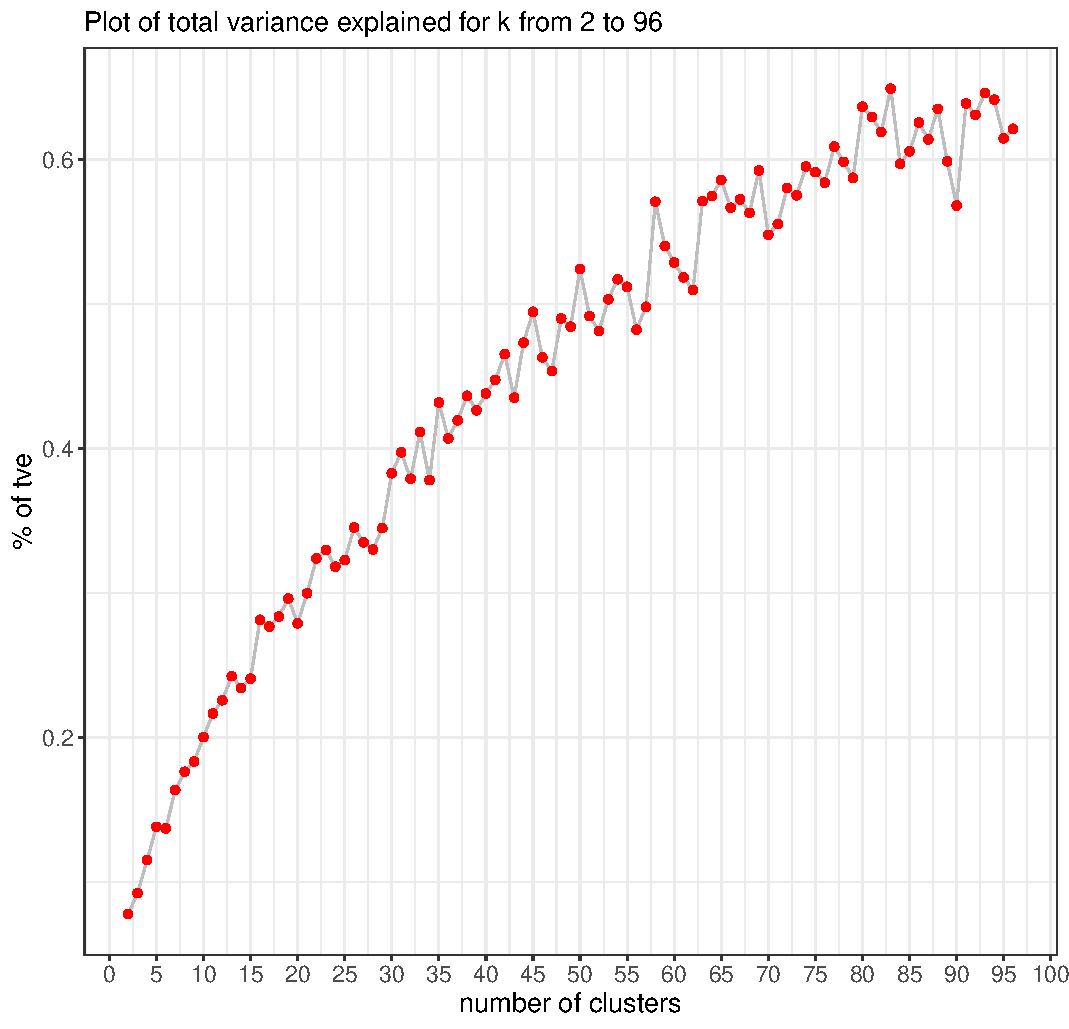
\includegraphics[width=0.7\textwidth, keepaspectratio]{numclusters.pdf} \\
\caption{Plot of the total variance explained against different values of \textit{k} \protect
\includegraphics[scale=0.05]{qletlogo.pdf} {\href{https://github.com/silvia-ventoruzzo/SPL-WISE-2018/blob/master/Helpers/number_of_clusters.R}{number\_of\_clusters.R}}}
\label{figure:numclusterplot}
\end{center}
\end{figure}

\subsection{k-means clustering}\label{subsec:kmeans}

After selecting the number of clusters to use, one can apply it inside the function \texttt{kmeans} and look at the cluster assignments of the different points.

Having multiple variables, plotting the clustered points with respect to all variables is not feasible, one need therefore to find alternatives. Since we have coordinate points, one possibility is to plot the points with respect to their longitude and latitude, like in figure \ref{figure:cluster_map}. Another one can be to plot them with respect to the first two principal components, as in figure \ref{figure:cluster_plot}.

\begin{figure}[H]
\centering
\subfloat[With respect to the coordinates]{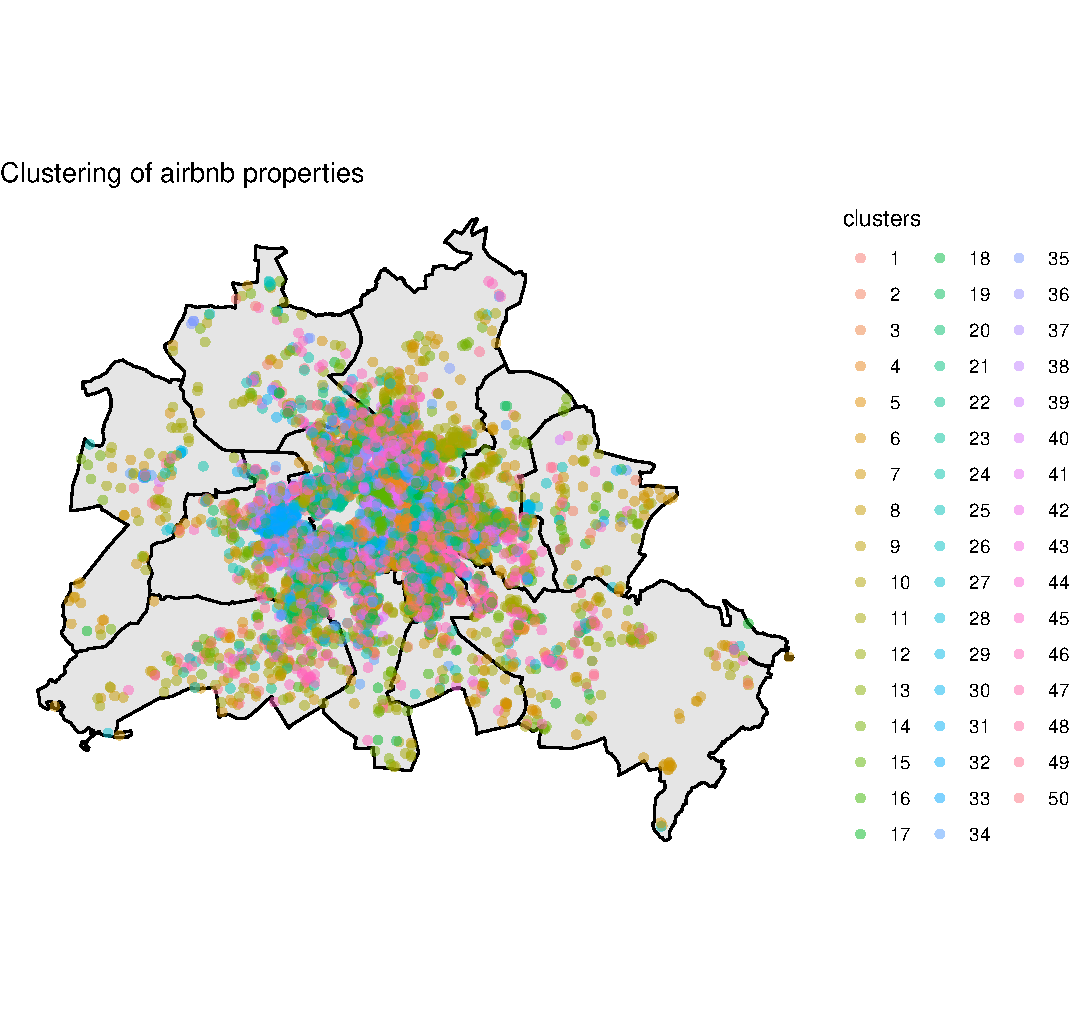
\includegraphics[height=0.5\textwidth]{cluster_map.pdf}
\label{figure:cluster_map}}
\subfloat[With respect to Principal Components]{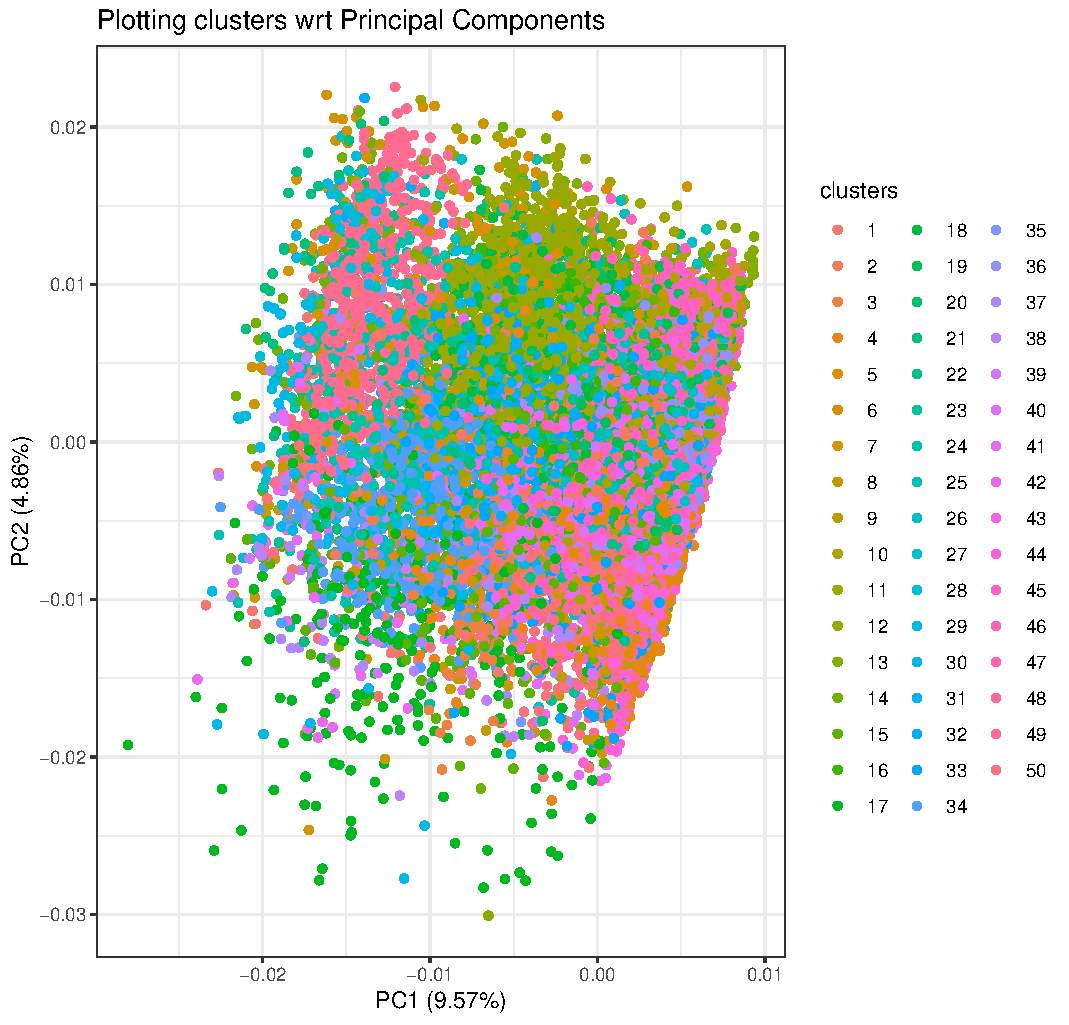
\includegraphics[height=0.5\textwidth]{cluster_plot.pdf}
\label{figure:cluster_plot}}
\caption{Plotting the clusters}
\centering
\end{figure}

Because of the large amount of variables, points and clusters, it is not easy to visually display the groups. This task can be left for further studies.